\documentclass[11pt]{article}
\usepackage[margin=1in]{geometry}
\usepackage[T1]{fontenc}
\usepackage[utf8]{inputenc}
\usepackage{lmodern,microtype}
\usepackage{amsmath,amssymb,amsthm,mathtools}
\usepackage{graphicx,booktabs,array,enumitem,setspace,placeins}
\usepackage{algorithm}
\usepackage{algpseudocode}
\usepackage{needspace}
\usepackage[authoryear,round]{natbib}
\usepackage{xr-hyper}
\usepackage[colorlinks=true,allcolors=blue]{hyperref}
\usepackage{bookmark}
\allowdisplaybreaks
\setstretch{1.18}
\setlength{\parskip}{0pt}
\setlength{\emergencystretch}{2em}
\setlist{itemsep=2pt,topsep=4pt}
\newtheorem{theorem}{Theorem}[section]
\newtheorem{lemma}[theorem]{Lemma}
\newtheorem{proposition}[theorem]{Proposition}
\newtheorem{corollary}[theorem]{Corollary}
\newtheorem{definition}[theorem]{Definition}
\newtheorem{example}[theorem]{Example}
\theoremstyle{remark}
\newtheorem{remark}[theorem]{Remark}
\newcommand{\E}{\mathbb E}
\newcommand{\Prob}{\mathbb P}
\newcommand{\ind}{\mathbf 1}
\newcommand{\kl}{\operatorname{kl}}
\newcommand{\pos}[1]{\left[#1\right]_+}
\newcommand{\suppproof}{Complete proofs appear in the supplementary material.}

\hypersetup{pdftitle={Supplement to The Cost of Reliable Near-Optimal Set Maintenance with Arriving Arms},pdfauthor={}}
\renewcommand{\thesection}{S\arabic{section}}
\renewcommand{\thepage}{S-\arabic{page}}
\title{Supplement to ``The Cost of Reliable Near-Optimal Set Maintenance with Arriving Arms''}
\author{}
\date{October 15, 2026}
\begin{document}
\maketitle
\section*{Notation and scope}
The observation model has independent arm streams, each consisting of
independent, identically distributed rewards in $[0,1]$, deterministic
permanent arrivals $\mathcal A_t$, and one observation per physical time step.
Each finite $\mathcal A_t$ is nonempty, and arbitrarily large finite batches
are allowed. Arrivals occur before the action, and reports follow its
observation. Let $r^*(t)=\max_{i\in\mathcal A_t}r_i$,
$\Delta_i(t)=r^*(t)-r_i$, and
$\mathcal G_t^\varepsilon=\{i\in\mathcal A_t:\Delta_i(t)\le\varepsilon\}$.
Reports partition $\mathcal A_t$ as
$(\mathcal P_t,\mathcal N_t,\mathcal V_t)$. Write
\[
 E_{\rm lab}=\{\forall t:\mathcal P_t\subseteq\mathcal G_t^\varepsilon
                      \subseteq\mathcal A_t\setminus\mathcal N_t\},\qquad
 \mathcal U_T(\eta)=\sum_{t\le T}\sum_{i\in\mathcal A_t}
 \ind\{i\in\mathcal V_t,|\Delta_i(t)-\varepsilon|>\eta\},
\]
and $R_T=\sum_{t\le T}\Delta_{I_t}(t)$. Reliability means
$P(E_{\rm lab})\ge1-\delta$ for every allowed environment.
$\mathfrak R_\Theta(a)$ minimizes worst-case $ER_T$ over full-model reliable
policies with $P_\theta(E_{\rm lab},\mathcal U_T\le a)\ge1-\delta$ for all
$\theta\in\Theta$. A bar denotes averaging under the independent uniform
prior on all candidate signs. These priors are proof devices and impose no
Bayesian requirement on the policy.

The probability and sample-budget arguments are given below. Classical
change of measure and multiple-recovery scales are credited to the existing
literature \citep{kaufmann2016,malloy2014,jamieson2018,mason2020}.

% Reorganized from the frozen October 15, 2026 supplement.
\section{Probability tools and reporting conventions}
\label{app:tools}

For the reporting constructions, index arms in arrival order
$i=1,2,\ldots$, with a fixed order within each batch.
Every arm has an independent potential reward stream $(Y_{i,n})_{n\ge1}$
in $[0,1]$. The policy observes its $n$th entry on its $n$th pull. Arrival
times are deterministic, and reports are issued after the current observation.
Write $N_i(t)$ for lifetime observations through round $t$ and
$\hat r_i(n)=n^{-1}\sum_{s\le n}Y_{i,s}$. The observed reward in physical-time notation is
$X_{t,I_t}=Y_{I_t,N_{I_t}(t-1)+1}$. The conclusions below also
hold conditionally on an independent exogenous arrival schedule.

For independent $[0,1]$ observations, Hoeffding's inequality gives
\[
 P\{|\hat r_i(n)-r_i|>x\}\le2e^{-2nx^2}.
\]
For completeness, the centered log moment generating function has value and
derivative zero at the origin; its second derivative is a variance under an
exponentially tilted distribution and is at most $1/4$. Integrating twice
gives $Ee^{\lambda(X-EX)}\le e^{\lambda^2/8}$. Multiplication over independent
observations and exponential Markov inequality prove the display.

With
\[
 b_i(n)=\sqrt{\frac{\log(8i^2n^2/\delta)}{2n}},
\]
the union of all potential-prefix failures has probability at most
$\delta\zeta(2)^2/4<\delta$. Intersecting the prefix intervals with $[0,1]$
therefore gives simultaneous coverage. On that event each endpoint differs
from its mean by at most $2b_i(n)$. No conditioning on a previously selected
empirical mean is used. Empty intersections on failure paths are handled by
exclusion-first reporting; the reward policy remains defined on all paths.

The checkpoint alternative fixes, before observing arm $i$,
\[
 q_i(\rho_i)=\left\lceil\frac2{\rho_i^2}
            \log\frac{4i(i+1)}\delta\right\rceil.
\]
Before $q_i$ observations its interval is $[0,1]$; afterwards it is permanently
\[
 [\hat r_i(q_i)-\rho_i/2,
  \hat r_i(q_i)+\rho_i/2]\cap[0,1].
\]
The sum of coverage failures is at most
$\sum_i\delta/\{2i(i+1)\}=\delta/2$. On coverage, each endpoint differs from
the true mean by at most $\rho_i$. These intervals are nonempty on every path
and only contract once. If $\underline r^*(t)=\max_i\ell_i(t)$ and
$\overline r^*(t)=\max_i u_i(t)$, use
\[
 \mathcal P_t=\{i:\ell_i(t)\ge\overline r^*(t)-\varepsilon\},\quad
 \mathcal N_t=\{i:u_i(t)<\underline r^*(t)-\varepsilon\},\quad
 \mathcal V_t=\mathcal{A}_t\setminus(\mathcal P_t\cup \mathcal N_t).
\]
The sets $\mathcal P_t,\mathcal N_t$ are disjoint because
$\underline r^*(t)\le\overline r^*(t)$ and $\ell_i\le u_i$.
Coverage implies
$\mathcal P_t\subseteq \mathcal G_t^\varepsilon\subseteq \mathcal{A}_t\setminus \mathcal N_t$.
Moreover, $\mathcal N_t$ is increasing as observations and arrivals accumulate:
$\underline r^*(t)$ cannot decrease and an existing $u_i$ cannot increase.

For two Bernoulli mean vectors $\boldsymbol r=(r_i)_i$ and
$\boldsymbol r'=(r_i')_i$ and a bounded stopping time $\tau$, action
kernels, policy randomization, and stopping kernels cancel in the history
likelihood ratio. Padding after stopping by null symbols and taking iterated
expectations yields
\begin{equation}
 D(P_{\boldsymbol r}^{H_\tau}\Vert P_{\boldsymbol r'}^{H_\tau})
 =\sum_iE_{\boldsymbol r} N_i(\tau)\operatorname{kl}(r_i,r_i').
 \label{eq:app_kl_identity}
\end{equation}
The same proof applies to arbitrary observation laws with finite two-way KL.
For an event $F$ measurable at stopping, splitting the likelihood integral
over $F,F^c$ and applying Jensen gives
\[
 D(P\Vert Q)\ge\operatorname{kl}(P(F),Q(F))
 \ge P(F)\log\frac1{Q(F)}-\log2.
\]
The second inequality uses the binary entropy bound $h(p)\le\log2$. We repeatedly use
\[
 2(p-q)^2\le\operatorname{kl}(p,q)
 \le\frac{(p-q)^2}{q(1-q)}.
\]
The upper bound follows from $\log x\le x-1$; for the lower bound the second
derivative in $p$ is $1/\{p(1-p)\}\ge4$ and both value and derivative vanish
at $p=q$.

% Reorganized from the frozen October 15, 2026 supplement.
\section{Joint guarantee of Checkpoint-UCB}
\label{app:joint}

Checkpoint-UCB fixes each arm's checkpoint before seeing its data. At even
physical rounds it samples the earliest-arriving arm below its lifetime
checkpoint, if one exists. At all other rounds it maximizes, over every
available arm including reported exclusions,
\[
 J_i(t)=\hat r_i(N_i(t-1))+
             \sqrt{3\log(2t)/N_i(t-1)},
\]
with index $+\infty$ at zero count and deterministic ties. Every observation
serves both the lifetime checkpoint and the empirical reward estimate.
The fixed-checkpoint argument in Section~\ref{app:tools} gives
$P(E_{\rm lab})\ge1-\delta/2$. If $\mathcal I_T$ denotes designated
service rounds, then $|\mathcal I_T|\le\sum_{i\le K_T}q_i$, because each
such observation is charged to an arm below its single lifetime quota.
The following reward argument does not assume separated arrival windows.


\paragraph{A reward bound that does not condition on report coverage.}
At physical time $t$, order arms by their first observed rewards. At most
$t$ streams have been exposed, each at at most $t$ potential prefixes. A
previously unobserved stream is independent of the history selecting it.
Applying Hoeffding to each newly exposed stream and union bounding gives
\[
 P\left\{\exists\text{ observed arm and prefix }n\le t:
 |\hat r_i(n)-r_i|>
        \sqrt{3\log(2t)/n}\right\}
 \le2t^2(2t)^{-6}=\frac1{32t^4}.
\]
The exposure order is used only for this union bound, not to assert
independence among observed counts. An ordinary UCB pull with finite index,
on this event's complement, has
$\Delta_{I_t}(t)\le2\sqrt{3\log(2t)/N_{I_t}(t-1)}$.
Each arm--pre-pull-count pair is charged at most once; interleaved service
observations skip counts. Therefore the ordinary, nonfirst-pull regret is
at most
\[
 4\sqrt{3\log(2T)}\sum_i\sqrt{N_i(T)}
 \le4\sqrt{3K_TT\log(2T)}
\]
on good rounds. First pulls cost at most $K_T$, and the sum of expected
bad-round losses is less than one. Adding the actual regret of service
rounds proves
\[
 ER_T\le\min\left\{T,K_T+4\sqrt{3K_TT\log(2T)}+1+
       E\sum_{t\in\mathcal I_T}\Delta_{I_t}(t)\right\}.
\]
There is no $\delta T$ term: the reward policy never permanently discards an
arm because of a reporting error.


\begin{lemma}[Completion under arbitrary arrivals]
\label{app:completion_general}
Fix $0<\eta<1$ and use Checkpoint-UCB with the predetermined precision
$\rho=\eta/4$. Let $\overline Q_t$ be the post-service workload of the
virtual FIFO queue that inserts $q_i$ units at arm $i$'s arrival and serves
one unit at every even physical round when nonempty. On the simultaneous
checkpoint-coverage event, for each fixed deterministic endpoint $T$,
\[
 \mathcal U_T(\eta)\le
 \sum_{t\le T}K_t1\{\overline Q_t>0\}
 \le\min\{K_TT,2K_T\sum_{i\le K_T}q_i\}.
\]
\end{lemma}
\begin{proof}
If all current checkpoints are complete, all endpoint errors are at most $\eta/4$ and every arm whose
boundary distance exceeds $\eta$ has a determinate report. A virtual FIFO
queue adding $q_i$ work at each arrival and serving one unit at every even
round dominates unfinished checkpoints; additional UCB observations only
reduce actual work. Its busy periods, including alignment to the first even
round, have total length at most $2\sum_iq_i$. Thus on simultaneous coverage the unresolved area is bounded by the
queue-weighted sum in the statement, which is at most $K_TT$ and at most
$2K_T\sum_{i\le K_T}q_i$.
\end{proof}

% Reorganized from the frozen October 15, 2026 supplement.
\section{Broadcast uncertainty and queue area}
\label{app:broadcast}

\paragraph{Precise claim.}
Let $0<\varepsilon\le1/16$, $0<\delta\le1/16$,
$0<\eta<\varepsilon/2$. The reference arm has mean
$1/4+\varepsilon/2$. All candidates have mean $p=1/4$ in environment zero;
environment $j$ raises only candidate $j$ to $p+2\varepsilon$. Let $M_t$ be
the candidate count, $a_t$ the new-candidate count, and
\[
 q_- =\left\lfloor\frac{\operatorname{kl}(1/4,\delta)}
                         {\operatorname{kl}(1/4,1/4+2\varepsilon)}\right\rfloor,
 \quad Q_t=(Q_{t-1}+q_-a_t-1)_+,\quad Q_0=0,
\]
\[
 \mathcal B_T=\sum_{t\le T}(M_t-1)_+1\{Q_t>0\}.
\]
Every policy reliable on these environments obeys
\[
 E_0\mathcal U_T(\eta)\ge(3/4-\delta)\mathcal B_T,
 \qquad
 P_0\{\mathcal U_T(\eta)\ge\mathcal B_T/4\}\ge1/4
\]
when $\mathcal B_T>0$.

\begin{proof}
The denominator defining $q_-$ is at most
$\operatorname{kl}(1/4,3/8)\le1/15$, whereas its numerator is at least
$\frac14\log4+\frac34\log(4/5)\ge7/48>2/15$. Thus $q_-\ge2$.
The recursion gives, by induction,
\[
 Q_t=\max_{0\le u\le t}\left\{
       q_-\sum_{r=u+1}^ta_r-(t-u)\right\}.
\]
If $Q_t>0$, there is a suffix in which total candidate demand exceeds all
physical observation slots. Its arms had no observations before that suffix.
Consequently at least one deterministic candidate label $j$ satisfies
$E_0N_j(t)<q_-$. The choice is made from expected counts, not from a realized
history. For any other candidate $i$, membership of $i$ in $\mathcal P_t$ is erroneous
under environment $j$. Its probability there is at most $\delta$.
The history KL is strictly below $\operatorname{kl}(1/4,\delta)$, so data
processing and monotonicity of binary KL force $P_0(i\in \mathcal P_t)<1/4$.
Since all candidates are genuinely good under environment zero,
$P_0(i\in \mathcal N_t)\le\delta$. It follows that
$P_0(i\in \mathcal V_t)\ge3/4-\delta$. These candidates all have boundary distance
$\varepsilon/2>\eta$. Summing at deterministic busy rounds proves the
expectation bound, entirely under the one environment zero.

Let $Y$ count candidate unresolved area only at busy rounds with $M_t\ge2$.
Then $Y\le\mathcal U_T$, $0\le Y\le2\mathcal B_T$, and
$E_0Y\ge11\mathcal B_T/16$. If
$p=P_0(Y\ge\mathcal B_T/4)$, then
$11\mathcal B_T/16\le\mathcal B_T/4+(7\mathcal B_T/4)p$, so $p\ge1/4$.
\end{proof}

\paragraph{Queue area.}
For an integer $q\ge2$, suppose $m$ candidates arrive by time $s$ and put
$D=s+qm-1$. Then
\[
 \sum_{t\le D}(M_t-1)_+1\{Q_t(q)>0\}
 \ge\frac{q-1}{2}m(m-1).
\]
To prove this, remove all subsequent arrivals, which can only decrease both
the queue and its weights. The $qm$ service units finish by $D$. At the
$n$th actual service, at least $\lceil n/q\rceil$ candidates have arrived,
so service rounds weighted by $M_t-1$ sum to at least
$\sum_{n=1}^{qm}(\lceil n/q\rceil-1)=qm(m-1)/2$.
The post-service queue is zero at the last service round of each busy period.
Their cumulative arrival counts are distinct integers in $\{1,\ldots,m\}$,
so removing their weights costs at most $m(m-1)/2$. This proves the claim.

In particular, if along a fixed infinite schedule a policy reliable in every
environment has a deterministic area envelope $a_T=o(T)$, then
$K_t=o(\sqrt t)$. Otherwise along $s_n$ there are at least $c\sqrt{s_n}$
candidates. Choose the first $m_n=\lfloor c\sqrt{s_n}\rfloor$; eventually
$q_-m_n\le s_n$. The queue bound and the preceding probability statement at
$2s_n$ give $P_0(\mathcal U_{2s_n}\ge c's_n)\ge1/4$, contradicting
$\delta\le1/16$ and the proposed envelope.

% Reorganized from the frozen October 15, 2026 supplement.
\section{Partial simultaneous recovery}
\label{app:partial}

\paragraph{Precise claim.}
Let $m\ge1$ independent uniform signs specify independent observation laws
$P_i^+,P_i^-$. All nuisance parameters and observations are independent of
these signs. Sampling may be adaptive and interleaved, and $\tau$ is bounded.
At every sign configuration, the probability of any erroneous determinate
report is at most $\delta\le1/16$. Let $J_\tau$ be the number of determinate
reports and
$\kappa=\max_i\max\{D(P_i^+\Vert P_i^-),D(P_i^-\Vert P_i^+)\}\in(0,\infty)$.
If $\overline P(J_\tau\ge m/2)\ge1/2$, then
\[
 \overline E\sum_iN_i(\tau)\ge\frac{m}{1024\kappa}\log\frac m\delta.
\]

\begin{proof}
Let $L_i$ be the observed positive-versus-negative log likelihood ratio for
coordinate $i$. After conditioning on the full stopped history, the action
and stopping kernels cancel. The likelihood factors over coordinates and so
does the posterior, even though the sample counts need not be independent.
The smallest coordinatewise posterior error is
$e_i=(1+e^{|L_i|})^{-1}$. If $S$ is the reported subset, its conditional
probability of complete correctness is at most $\prod_{i\in S}(1-e_i)$;
choosing a non-MAP label cannot improve it. Thus
\[
 \overline E\left[1-\prod_{i\in S}(1-e_i)\right]\le\delta.
\]
With probability at least $1-2\delta$ this product is at least $1/2$ and hence
$\sum_{i\in S}e_i\le\log2$. Intersecting with $J_\tau\ge m/2$ costs at most
$2\delta$ and leaves probability at least $3/8$. For $m\ge4096$, Jensen gives
on this intersection
\[
 \sum_i|L_i|\ge\sum_{i\in S}\{\log(1/e_i)-\log2\}
 \ge\frac m2\log\frac{m}{4\log2}.
\]
Successive conditional expectations of signed likelihood increments give
\[
 \overline E\sum_i\sigma_iL_i\le\kappa\overline E\sum_iN_i(\tau).
\]
Finite two-way KL makes the stopped increments integrable. Given the history,
$E(\sigma_iL_i\mid H_\tau)=|L_i|(1-2e_i)$, and
$2|L_i|e_i\le1$ for every real $L_i$. Therefore
\[
 \kappa\overline E\sum_iN_i\ge\overline E\sum_i|L_i|-m
 \ge m\left\{\frac3{16}\log\frac{m}{4\log2}-1\right\}
 \ge\frac m{256}\log m,
\]
where the last inequality holds for $m\ge4096$.

For the confidence term, fix a sign vector and flip coordinate $i$ only.
The event reporting the original sign on coordinate $i$ has original
probability at least its determinate-report probability minus $\delta$, and
flipped probability at most $\delta$. Average the data-processing inequalities
over vectors and coordinates and use joint convexity of binary KL.
Since $\overline EJ_\tau\ge m/4$, this yields
\[
 \kappa\overline E\sum_iN_i\ge
 m\operatorname{kl}(1/4-\delta,\delta)
 \ge\frac m{256}\log(1/\delta).
\]
To check the last scalar inequality, write $L=\log(1/\delta)$. For $L\le8$,
Pinsker gives a lower bound $2(1/4-2\delta)^2\ge1/32\ge L/256$.
For $L\ge8$, binary entropy at most $\log2$ gives
$\operatorname{kl}(1/4-\delta,\delta)\ge3L/16-\log2\ge L/16$.
When $m\ge4096$, the maximum of the two preceding bounds is at least half
their sum. When $m<4096$, $\log m\le3\log(1/\delta)$, and the confidence
bound alone suffices. Both cases imply the stated constant $1/1024$.
\end{proof}

\paragraph{Single-window truncation.}
If such a batch has $H$ rounds with qualifying boundary distance larger than
$\eta$, set
\[
 h_* =\min\left\{H,
 \left\lceil\frac{m\log(m/\delta)}{1024\kappa}\right\rceil-1\right\}.
\]
At every $r\le h_*$ there are at most $r$ batch observations. The recovery
lemma's contrapositive makes the probability of half-completion less than
$1/2$, so the expected unresolved count is at least $m/4$. Thus batch area
has expectation at least $mh_*/4$. Its first-$h_*$-round area $Y$ lies in
$[0,mh_*]$; consequently
$\overline P(Y\ge mh_*/8)\ge1/7$. One fixed sign configuration attains
at least this probability. If $h_*=0$, only the trivial zero lower bound is
asserted.

% Reorganized from the frozen October 15, 2026 supplement.
\section{Worst-schedule area and growth consequences}
\label{app:worst_area}

Suppose $0<\varepsilon\le1/8$, $0<\eta\le\varepsilon/32$,
$0<\delta\le1/16$, and $K\ge2$. Let $\mathfrak A_{T,K}$ be the smallest
area threshold attainable with joint label-and-area probability at least
$1-\delta$, uniformly over reward environments and schedules with $K_T\le K$.
The policy must be reliable on the full model.

\paragraph{Upper bound.}
Use fixed precision $\rho=\eta/4$. Then
\[
 q_i=\left\lceil32\eta^{-2}\log\frac{4i(i+1)}\delta\right\rceil
 \le99\eta^{-2}\log(K/\delta),\qquad i\le K.
\]
Lemma~\ref{app:completion_general} proves, on coverage,
\[
 \mathcal U_T\le\min\{KT,2K\sum_{i\le K}q_i\}
 \le256\min\{KT,K^2\eta^{-2}\log(K/\delta)\}.
\]
The unconditional reward bound in Section~\ref{app:joint} and at most $\sum_iq_i$ service pulls also give
\[
 ER_T\le\min\{T,K+4\sqrt{3KT\log(2T)}+1+
                  99K\eta^{-2}\log(K/\delta)\}.
\]

\paragraph{Lower bound.}
At round one release a reference of mean $1/2+\varepsilon$ and
$m=K-1$ candidates of means $1/2\pm2\eta$. Their signs are independent and
specify their relative-goodness labels. The reference is always optimal;
its known distribution gives no sign information. Boundary distances equal
$2\eta>\eta$, and two-way KL is at most $128\eta^2$. Set
\[
 q_* =\frac{m\log(m/\delta)}{131072\eta^2},\qquad
 h=\min\{T,\lceil q_*\rceil-1\}.
\]
Since $\eta\le1/256$, $q_*\ge m\log(m/\delta)/2>1$ and
$h\ge\frac12\min\{T,q_*\}$. Single-window truncation gives a fixed
environment with
\[
 P\{\mathcal U_T\ge mh/8\}\ge1/7>\delta.
\]
Therefore no valid uniform area quantile can be smaller than
$m\min\{T,q_*\}/16$. The comparisons
$m\ge K/2$ and $\log(m/\delta)\ge\frac12\log(K/\delta)$ yield
\[
 \mathfrak A_{T,K}\ge
 2^{-24}\min\{KT,K^2\eta^{-2}\log(K/\delta)\}.
\]
The lower bound uses a static first-round burst; it does not attribute its
statistical logarithm uniquely to dynamic arrivals.

At fixed task parameters, uniformly over schedules satisfying a terminal
count limit $K_T\le k(T)$, sublinear expected regret and sublinear area
envelopes are simultaneously attainable if and only if
$k(T)^2\log k(T)=o(T)$. Necessity is the last lower bound; sufficiency follows
from the displayed upper bounds. This terminal-count-class conclusion
allows the worst schedule to depend on $T$.

\paragraph{Growth on a fixed schedule.}
At fixed $\eta,\delta$, the checkpoints are $O(\log(ei))$, so
$K_T^2\log(eK_T)=o(T)$ suffices for both sublinear area and expected regret.
Combined with the broadcast consequence in Section~\ref{app:broadcast}, a path with
$K_t\asymp t^\alpha$, $0<\alpha<1$, admits both if and only if $\alpha<1/2$.
This is an exponent statement and does not remove the critical logarithm.


\paragraph{A fixed sparse schedule that still defeats a uniform area envelope.}
Set
\[
 s_n=2^{2^n},\qquad
 m_n=\left\lfloor\frac{\sqrt{s_n}}{(\log s_n)^{1/4}}\right\rfloor.
\]
Release one reference at time one and $m_n$ candidates at each $s_n$.
Earlier batch sizes sum to $o(m_n)$, so $K_{s_n}/\sqrt{s_n}\to0$; between
batches the ratio decreases. Thus $K_t=o(\sqrt t)$ on this one schedule.
For each selected batch $n$, give the reference mean $1/2+\varepsilon$,
that batch means $1/2\pm2\eta$, and other candidates mean $1/2$. Let
\[
 h_n=\left\lceil\frac{m_n\log(m_n/\delta)}{131072\eta^2}\right\rceil-1,
 \qquad T_n=s_n+h_n-1.
\]
For large $n$, $h_n=o(s_n)$ and the next batch has not arrived. The old
history is independent of the new signs. Single-window truncation supplies
one fixed configuration for this endpoint with
$P(\mathcal U_{T_n}\ge m_nh_n/8)\ge1/7$. But
\[
 \frac{m_nh_n}{T_n}\asymp_{\eta,\delta}\sqrt{\log s_n}\longrightarrow\infty.
\]
No deterministic envelope $a_T=o(T)$ can consequently hold uniformly over
reward environments for this schedule. The reward environment may vary
with the chosen endpoint; this is exactly the uniform-in-environment
statement and is not a claim of simultaneous failure at all endpoints in
one fixed reward environment.

% Reorganized from the frozen October 15, 2026 supplement.
\section{Area-constrained temporary tasks}
\label{app:area_lower}

In window $e$, suppose $M_e$ candidates have gaps
$\varepsilon-\sigma_{e,k}d_e$, and a new reference makes their signs
irrelevant after that window. Put $w_e=M_eH_e$, $V=\sum_ew_e$, and let
$p_e$ be the product-prior probability that at least half of batch $e$ becomes
determinate simultaneously before its window ends. Define
\[
 \Phi_\delta(u)=
 \begin{cases}
  \operatorname{kl}(1-\delta-u,\delta),&u<1-2\delta,\\
  0,&u\ge1-2\delta,
 \end{cases}
\]
\[
 g_{m,\delta}(p)=\max\left\{0,
 \frac{(p-2\delta)_+}{2}
       \left[\log\frac m{4\log2}\right]_+-1,
 \Phi_\delta(1-p/2)\right\}.
\]
Each displayed component is convex and nondecreasing in $p$.

\begin{proof}[Proof of the general area-to-regret lower bound]
If window $e$ never half-completes, at every round more than half its
candidates remain unresolved. Its area is at least $w_e/2$. On area success,
$\sum_ew_e1_{S_e^c}\le2a$; outside that event this sum is at most $V$.
Consequently
\[
 \sum_ew_ep_e\ge(1-\delta)V-2a.
\]
Stop batch $e$ at first half-completion or at its endpoint. The likelihood
argument above now intersects the product-posterior event with completion
probability $p_e$, giving intersection probability at least
$(p_e-2\delta)_+$ and expected determinate count at least $M_ep_e/2$.
The absolute-likelihood and coordinate-flip derivations therefore give
\[
 \kappa_e\overline EN_e\ge M_eg_{M_e,\delta}(p_e).
\]
For the absolute-likelihood term, when the bracketed logarithm is positive
its Jensen expression is increasing for subset sizes at least $M_e/2$;
when it is nonpositive the stated term is at most zero. Each observation
counted before stopping has regret at least $\varepsilon-d_e$.
The signs of all batches belong to one product prior, and samples of
different batches are disjoint. Hence
\begin{equation}
\label{eq:allocation_lower}
 \sup_\sigma E_\sigma R_T\ge
 \inf_{\substack{0\le p_e\le1\\
       \sum_ew_ep_e\ge(1-\delta)V-2a}}
 \sum_e\frac{(\varepsilon-d_e)M_e}{\kappa_e}
                  g_{M_e,\delta}(p_e).
\end{equation}
This is an information lower relaxation, not a claim that every feasible
allocation is achieved by a causal policy.
\end{proof}

\paragraph{Homogeneous consequence.}
Take $M_e=M$, $H_e=H$, $d_e=d$, and $a=JMH/8$. On success at least $3J/4$
windows half-complete; thus $\sum_ep_e\ge45J/64$. At least $3J/8$ windows
have $p_e\ge1/2$: otherwise the sum is at most
$3J/8+(5J/8)/2=11J/16<45J/64$.
The Bernoulli means lie in $[1/4,3/4]$, giving $\kappa_e\le32d^2$.
The partial-recovery lemma and $\varepsilon-d\ge\varepsilon/2$ yield
\[
 \sup_\sigma E_\sigma R_T\ge
 \frac{3J}{8}\frac{\varepsilon M}{2\cdot1024\cdot32d^2}
             \log\frac M\delta
 \ge2^{-20}\frac{\varepsilon JM}{d^2}\log\frac M\delta.
\]

% Reorganized from the frozen October 15, 2026 supplement.
\section{Shared evidence and rapid/deferred endpoints}
\label{app:reuse}

\subsection{Shared evidence across separated windows}
Let batch $e$ have reference mean $b_e$, $M_e$ candidate means
$b_e-\varepsilon\pm d_e$, and common predetermined precision $\rho_e$.
The final batch contains only its reference; set $M_J=M_{-1}=0$ and
$S_e=\sum_{i\in F_e}q_i(\rho_e)$. Assume
\[
 H_e\ge2S_e,\quad b_J-b_0\le\varepsilon/4,\quad
 d_e+\rho_e+\rho_{e+1}<b_{e+1}-b_e,\quad
 2\max_e\rho_e\le\varepsilon/2.
\]
The algorithm is not told which arm is the reference or when the next window
starts. By induction every batch completes its checkpoints within its first
$2S_e$ rounds, before the next batch appears. On coverage, successive
reference levels satisfy $b_e+\rho_e<b_{e+1}-\rho_{e+1}$. Once batch $e$
completes, the maximum upper endpoint of all available arms is at most
$b_e+\rho_e$. Its candidates are therefore completely classified when
$2\rho_e<d_e$.

An old candidate in batch $e-1$ has upper endpoint at most
$b_{e-1}-\varepsilon+d_{e-1}+\rho_{e-1}$, whereas the new reference has
lower endpoint at least $b_e-\rho_e$. Their difference exceeds
$\varepsilon$, excluding the entire preceding candidate batch without any
further old-arm observations. Older exclusions persist. Every reference has
gap at most $\varepsilon/4$ and total endpoint error at most
$\varepsilon/2$, so all references become positively certified.
If $F=\{e<J:2\rho_e<d_e\}$, the area is consequently at most
\[
 \sum_{e\notin F}M_eH_e+2\sum_{e\in F}M_eS_e+
                2\sum_{e=0}^J(e+1+M_{e-1})S_e.
\]
The terms cover current nonfine candidates, fine candidates, and temporarily
unresolved references plus the preceding candidate batch. All earlier
candidate batches have already been excluded.

For expected regret, every observation with pre-pull count below $q_i$
occurs in its arm's birth window. Such reference observations have zero
regret, and candidate observations cost at most $\varepsilon+d_e$ each.
All observations with pre-pull count at least $q_i$ are ordinary UCB pulls.
For each arm that has a positive gap by $T$, let
$\gamma_i=\min_{t\le T:i\in\mathcal A_t,\,\Delta_i(t)>0}\Delta_i(t)$
and $D_i^T=\max_{t\le T:i\in\mathcal A_t}\Delta_i(t)$.
Use the good-round concentration bound from Section~\ref{app:joint}. At a good UCB round, any positive-gap
pull has pre-pull count at most $12\log(2T)/\gamma_i^2$. Since lifetime counts do not
repeat, this gives the unconditional bound
\begin{equation}
\label{eq:app_reuse_regret}
 ER_T\le\sum_{e<J}\sum_{k=1}^{M_e}(\varepsilon+d_e)q_{e,k}
 +\sum_{i:\gamma_i\text{ exists}}D_i^T
 \left[\left\lceil\frac{12\log(2T)}{\gamma_i^2}\right\rceil-q_i+1\right]_+
 +1.
\end{equation}
The completion-before-next-batch assumption is essential to the first
charging term. It is not an assertion about arbitrary overlapping arrivals.

\subsection{Rapid and deferred endpoints on one family}
\label{app:tradeoff}

Here $J\ge1$, $M\ge\max\{2,J\}$,
$0<\varepsilon\le1/8$, $0<\delta\le1/16$, $Jv\le\varepsilon/4$,
$0<d\le v/32$, and $\eta=d/2$. The reference means are
$b_e=1/2+ev$ and the $M$ candidates born in window $e<J$ have means
$b_e-\varepsilon+\sigma_{e,k}d$. Each window has length $H$, and the final
window contains only a new reference. Set
\[
 K=J(M+1)+1,\quad L_K=\log\frac{4K(K+1)}\delta,
 \quad q_f=\lceil32L_K/d^2\rceil,\quad q_c=\lceil128L_K/v^2\rceil,
\]
\[
 H=128(M+J+1)q_f,\qquad T=(J+1)H,\qquad V=JMH.
\]
These are analysis quantities: the policy uses the selected precision
$\rho_f=d/4$ or $\rho_c=v/8$, not $K,H,T$ or the best-arm identities.
Both choices satisfy the separated-window conditions.

The preceding area bound is at most $B_{J,M}q_f$ for the fine policy and
$V+B_{J,M}q_c$ for the coarse policy, where
\[
 B_{J,M}=2(M+1)\{J(2M+1)+J(J-1)/2\}+2(M+J+1).
\]
For $2\le M$ and $J\le M$, $B_{J,M}\le12JM^2$. Indeed,
$M+1\le3M/2$, $2M+1\le5M/2$, and $J-1\le M$ bound the main term by
$9JM^2$, and the final term by $3JM^2$. The definition of $H$ gives
$B_{J,M}q_f\le V/8$, while $q_c\le q_f$ gives coarse area at most $9V/8$.
Both statements hold on the same fixed-checkpoint coverage event of
probability at least $1-\delta/2$.

For rapid maintenance the area-to-regret lower bound applies. For its upper
bound, every available arm in this family has gap at most $2\varepsilon$.
Hence, on every path, $R_T\le2\varepsilon T$. Since
$(J+1)(M+J+1)/(JM)\le5$,
\[
 2\varepsilon T\le1280\varepsilon JM q_f.
\]
Furthermore $K\le2M^2$, $K+1\le3M^2$ imply
$L_K\le5\log(M/\delta)$, and
$q_f\le165d^{-2}\log(M/\delta)$. Thus
\[
 2^{-20}\frac{\varepsilon JM}{d^2}\log\frac M\delta
 \le\mathfrak R_\Theta(V/8)
 \le2^{18}\frac{\varepsilon JM}{d^2}\log\frac M\delta.
\]
This upper bound uses the stated horizon and must not be extended unchanged
to arbitrarily long windows.

For the coarse policy, within-checkpoint candidate regret is at most
$2\varepsilon JM q_c$. Candidates have
$\gamma_i\ge\varepsilon-d\ge3\varepsilon/4$, $D_i^T\le2\varepsilon$;
old references have $\gamma_i\ge v$, $D_i^T\le Jv$. Dropping the favorable
quota subtraction in \eqref{eq:app_reuse_regret} and absorbing integer terms
gives
\[
 \sup_\Theta ER_T\le2\varepsilon JM q_c+
 64\left(\frac{JM}{\varepsilon}+\frac{J^2}{v}\right)\log(2T)+1.
\]
At fixed $J,M,\varepsilon,v,\delta$, $d\downarrow0$ makes
$T=\Theta(d^{-2})$. Consequently the rapid endpoint is $\Theta(d^{-2})$
and the deferred endpoint is at most $O(\log(1/d))$. No matching lower bound
for the latter endpoint is asserted.

% Reorganized from the frozen October 15, 2026 supplement.
\section{Regret quantiles under the same maintenance protocol}
\label{sec:quantile_extension}

The following result strengthens the expectation lower bound. Its statement
uses the same reporting event and the same cumulative unresolved area; it does
not introduce a separate deadline requirement. Write $\overline P$ for the
product prior on all candidate signs in the repeated-update family.

\Needspace{14\baselineskip}
\begin{lemma}[Completion with a bounded candidate-sampling budget]
\label{lem:budget_completion}
Consider one batch of $m$ candidates in its validity window, under the
assumptions of the partial-recovery lemma. Let $\tau$ be the first round at
which at least $m/2$ candidates have determinate reports, or the end of the
window if this does not occur. Let $S$ denote that completion occurs, and let
$N(\tau)$ count only samples of this batch. Put
\[
 L=\frac{m\log(m/\delta)}{1024\kappa},\qquad
 q=\lfloor L/2\rfloor.
\]
If $L\ge4$, then
\[
 \overline P\{S,\ N(\tau)\le q\}<\frac12.
\]
\end{lemma}
\begin{proof}
Stop at the earliest of $\tau$, the window endpoint, and the first round with
$q+1$ candidate samples. At this bounded stopping time $\zeta$, the number of
candidate samples is at most $q+1<L$. On $\{S,N(\tau)\le q\}$, the budget
stopping condition has not fired before $\tau$, so $\zeta=\tau$ and at least
$m/2$ reports are determinate. If the displayed event had probability at least
$1/2$, the partial-recovery lemma at $\zeta$ would give
$\overline E N(\zeta)\ge L$, contradicting the deterministic bound
$N(\zeta)\le q+1<L$.

The extra sample in the stopping rule is needed. Stopping exactly at the
$q$th candidate sample would miss a completion that uses $q$ candidate
samples and later observations of the reference arm.
\end{proof}

\begin{theorem}[Regret quantiles required by rapid maintenance]
\label{thm:quantile_lower}
In the repeated-update family with $J$ validity windows, $M$ candidates per
window, $M\ge\max\{2,J\}$, $Jv\le\varepsilon/4$,
$d\le v/32$, $\eta=d/2$, and $0<\delta\le1/16$, suppose a policy is
$\delta$-reliable on the family and, for every sign configuration $\sigma$,
\[
 P_\sigma\{E_{\rm lab},\ \mathcal U_T(\eta)\le JMH/8\}\ge1-\delta.
\]
Then there is one fixed configuration $\sigma$ for which
\[
 P_\sigma\left\{R_T\ge
 2^{-20}\frac{\varepsilon JM}{d^2}\log\frac M\delta\right\}
 \ge\frac{11}{80}.
\]
This conclusion permits the policy to know the reference identities, the
arrival schedule, and the horizon.
\end{theorem}
\begin{proof}
Let $S_e$ denote completion of at least half of the current candidates before
the next reference arrives, and let $N_e$ be that batch's sample count at its
first such completion, or at the window endpoint when completion fails.
Set
\[
 L_0=\frac{M\log(M/\delta)}{32768d^2},\qquad
 q_0=\lfloor L_0/2\rfloor.
\]
The two directional Bernoulli divergences are at most $32d^2$, so the
partial-recovery lower bound is at least $L_0$. The assumptions imply
$d\le1/1024$ and $M\ge2$, hence $L_0>4$.
The preceding budget argument, with $q_0+1<L_0$, gives
\[
 \overline P(F_e)<\frac12,
 \qquad F_e:=\{S_e,N_e\le q_0\}.
\]
The argument is valid with all previous-window information included in the
history. Those observations and later reference distributions carry no
information about this batch's independent signs.

On the area-success event, any window without $S_e$ contributes at least
$MH/2$ area. Consequently $\sum_e1_{S_e}\ge3J/4$ on an event of prior
probability at least $1-\delta$. If $F=\sum_e1_{F_e}$, then
$\overline EF\le J/2$ and Markov's inequality gives
\[
 \overline P\{F\le5J/8\}\ge1/5.
\]
No independence across windows is asserted or needed. Intersecting these two
events has probability at least
$1/5-\delta\ge11/80$. On their intersection at least $J/8$ windows complete
with $N_e>q_0$, and therefore with $N_e>L_0/2$.
Each candidate observation in its birth window has gap at least
$\varepsilon-d\ge\varepsilon/2$. These are observations of distinct batches
in disjoint windows. Pathwise on that intersection,
\[
 R_T\ge\frac{\varepsilon}{2}\frac J8\frac{L_0}{2}
 =2^{-20}\frac{\varepsilon JM}{d^2}\log\frac M\delta.
\]
A mixture probability at least $11/80$ implies that one fixed configuration
has at least that probability. Thus no different worst environment is selected
for different windows.
\end{proof}

\begin{corollary}[Rapid maintenance with a joint regret quantile]
\label{cor:joint_quantile}
Let $\mathfrak R^{\rm joint}_\Theta(a)$ be the infimum of $r$ over policies
that are reliable on the full bounded model and satisfy
\[
 \inf_{\theta\in\Theta}
 P_\theta\{E_{\rm lab},\mathcal U_T(\eta)\le a,R_T\le r\}\ge1-\delta.
\]
For the repeated-update horizon
$H=128(M+J+1)\lceil32d^{-2}\log\{4K(K+1)/\delta\}\rceil$,
where $K=J(M+1)+1$, universal positive constants $c,C$ satisfy
\[
 c\frac{\varepsilon JM}{d^2}\log\frac M\delta
 \le\mathfrak R^{\rm joint}_\Theta(JMH/8)
 \le C\frac{\varepsilon JM}{d^2}\log\frac M\delta.
\]
\end{corollary}
\begin{proof}
For the lower bound, every policy feasible for the joint criterion satisfies
the area premise of Theorem~\ref{thm:quantile_lower}. Since
$11/80>\delta$, a joint regret bound strictly below its threshold is
impossible. Taking an infimum gives the claimed lower bound.
For the upper bound, the fine-checkpoint policy has the required area bound
on its simultaneous interval-coverage event, whose probability is at least
$1-\delta/2$. Independently of coverage, every available arm in the family has
gap at most $2\varepsilon$, so $R_T\le2\varepsilon T$ on every sample path.
The specified horizon and $J\le M$ yield the displayed upper order, with the
same universal constant as the rapid-maintenance upper bound.
\end{proof}

% Reorganized from the frozen October 15, 2026 supplement.
\section{Compatible-window truncated area}
\label{sec:truncated_extension}

\begin{proposition}[Additive truncated area in one compatible experiment]
\label{prop:truncated_windows}
Consider finitely many batches indexed by $e$. Batch $e$ contains $m_e$
independent signs and has a deterministic validity window $W_e$ of length
$H_e$ that begins at that batch's arrival round. During that window each sign
is its arm's relative-goodness label and
its boundary distance exceeds $\eta$. The signs across all batches are
independent, other distributions do not encode them, and no information
about batch $e$ is available before its arrival. Samples remain interleaved
and adaptive. Suppose every sign configuration has familywise reporting error
at most $0<\delta\le1/16$. Let $0<\kappa_e<\infty$ bound the two directional
divergences in batch $e$, and define
\[
 h_e=\min\left\{H_e,
 \left\lceil\frac{m_e\log(m_e/\delta)}{1024\kappa_e}\right\rceil-1\right\},
 \qquad S=\sum_e m_eh_e.
\]
When $S>0$, one fixed full sign configuration satisfies
\[
 P\{\mathcal U_T(\eta)\ge S/8\}\ge1/7,
\]
provided every selected window lies before $T$ and every candidate--time pair
is counted only once. The windows may overlap when they concern distinct
arms and their stated qualification structure is jointly realizable.
\end{proposition}
\begin{proof}
At the $r$th round after batch $e$ arrives, $r\le h_e$, the entire experiment
has supplied at most $r$ samples of that batch. The contrapositive of the
partial-recovery lemma shows that at least half the batch is determinate with
probability less than $1/2$. Its expected unresolved count is therefore at
least $m_e/4$. Let $Y$ sum unresolved candidate--time pairs over the first
$h_e$ rounds of all selected windows. All these pairs have boundary distance
larger than $\eta$, so $Y\le\mathcal U_T(\eta)$, while $0\le Y\le S$ and
$\overline EY\ge S/4$. If $p=\overline P(Y\ge S/8)$, then
$S/4\le S/8+(7S/8)p$, giving $p\ge1/7$. Select a fixed configuration from
the common product prior. Compatibility of the windows is essential: this
proof cannot sum bounds from mutually incompatible reference environments.
\end{proof}

% Reorganized from the frozen October 15, 2026 supplement.
\section{Eventual exact classification and unconditional regret}
\label{app:consistency}

This extension uses a separate, revisable multiresolution policy, rather
than the fixed-checkpoint policy. Let epochs be $E_e=\{16^e,\ldots,16^{e+1}-1\}$ and use cumulative targets
$q_e=\lceil4^e(e+1)^2\rceil$. At even rounds serve, by FIFO, any arrived
arm below the current target, including arms formerly reported excluded.
Other rounds use full-history UCB. In epoch $e$ report from the raw intervals
with radius
\[
 b_{i,e}(n)=\sqrt{\frac{\log\{16i^2(e+1)^2n^2/\delta\}}{2n}},
\]
clipped to $[0,1]$ and equal to $[0,1]$ at zero count. Intervals are
recomputed rather than permanently intersected across epochs.

Hoeffding and a union over $i,e,n$ bound the probability of any coverage
failure by $\delta\zeta(2)^3/8<\delta$. This proves all-time reporting
reliability. Suppose arrivals eventually stop with $K<\infty$. For all large
$e$, the current epoch's remaining checkpoint work is at most $Kq_e$, and
its $2Kq_e$ physical service time is smaller than $15\cdot16^e$. Therefore
each arm has at least $q_{e-1}$ observations at the beginning of every
sufficiently late epoch. Uniformly for $t\in E_e$ and actual
$n\in[q_{e-1},t]$, the radius is
$O(\sqrt{\{e+\log i+\log(1/\delta)\}/q_{e-1}})=o(1)$.

For every positive rational $z$, Hoeffding makes
$\sum_nP(|\hat r_i(n)-r_i|>z)<\infty$. Tail union bounds imply only
finitely many deviations of size $z$ almost surely. Taking a countable
intersection over $z$ and the finitely many final arms gives simultaneous
empirical-mean convergence. If
$\min_i|\max_jr_j-r_i-\varepsilon|>0$, then all interval comparisons
are eventually correct and complete, almost surely. This conclusion is not
conditioned on early coverage, and early reporting errors can be corrected.

Through $T\in E_e$, service pulls number at most $Kq_e$, because targets are
cumulative and lifetime counts never decrease. This is
$O(K\sqrt T(1+\log T)^2)$. Apply the unconditional UCB counting bound in Section~\ref{app:joint} to
the remaining pulls to obtain
\[
 ER_T=O\{K\sqrt T(1+\log T)^2+\sqrt{KT\log(2T)}\}=o(T)
\]
for each eventually finite instance. Exact boundary cases are not included
in the complete-classification claim.

% Reorganized from the frozen October 15, 2026 supplement.
\section{General information-allocation relaxation}
\label{app:information}

This result is useful beyond the separated family, but does not assert
attainability. Fix a reference environment $\boldsymbol r$, endpoint $T$, and a
deterministic query set
\[
 \mathcal Q\subseteq\{(i,t):i\in \mathcal{A}_t,
                  |\Delta_i(t)-\varepsilon|>\eta\},\qquad W=|\mathcal Q|.
\]
For each query choose any allowed alternative $\boldsymbol r'$ that reverses arm
$i$'s membership at time $t$. Put $u_{i,t}=P_{\boldsymbol r}(i\in \mathcal V_t)$ and
\[
 \Phi_\delta(u)=
 \begin{cases}
 \kl(1-\delta-u,\delta),&0\le u<1-2\delta,\\
 0,&1-2\delta\le u\le1.
 \end{cases}
\]
This function is convex and nonincreasing: the positive branch is an affine
composition of binary KL, and its value and derivative vanish at the join.

\begin{proposition}[One protocol for area and information]
\label{prop:information}
For any reliable policy,
\[
 \sum_jE_{\boldsymbol r} N_j(t)\kl(r_j,r_j')
                       \ge\Phi_\delta(u_{i,t}).
\]
If its joint area budget at $\boldsymbol r$ is $a$, then
$\sum_{(i,t)\in\mathcal Q}u_{i,t}\le a+\delta W$. Consequently $E_{\boldsymbol r} R_T$
is at least the value of
\[
 \inf_{x,u}\sum_{s\le T}\sum_{j\in \mathcal{A}_s}\Delta_j(s)x_{s,j},
\]
subject to $x_{s,j}\ge0$, $\sum_{j\in \mathcal{A}_s}x_{s,j}=1$, no prearrival
allocations, the preceding unresolved-probability constraint, and for every
query and chosen alternative,
\[
 \sum_{s\le t}\sum_jx_{s,j}\kl(r_j,r_j')
                             \ge\Phi_\delta(u_{i,t}).
\]
For non-Bernoulli laws replace binary arm divergences by their distributional KL.
\end{proposition}
\begin{proof}
Let $F$ be the event of issuing, at $(i,t)$, the determinate label correct in
the reference environment. Then $P_{\boldsymbol r}(F)\ge1-u_{i,t}-\delta$, whereas
$P_{\boldsymbol r'}(F)\le\delta$. The history-KL identity and data processing give
the claimed constraint whenever $1-u_{i,t}-\delta>\delta$; otherwise
nonnegativity suffices. This is the precise point where the truncated KL is
needed. On area success the queried unresolved sum is at most $a$; outside
success it is at most $W$. Taking expectations gives $a+\delta W$.
The actual occupation probabilities $x_{s,j}=P_{\boldsymbol r}(I_s=j)$ satisfy every
constraint, with objective exactly $E_{\boldsymbol r} R_T$.
\end{proof}

One observation can enter many information constraints but is charged once
in the objective. Neither convex feasibility nor an oracle allocation proves
that a policy with unknown means and future arrivals attains this relaxation.
Dropping $\delta W$ would also change the stated risk protocol.

% Reorganized from the frozen October 15, 2026 supplement.
\section{Intermediate service configurations and disclosed-reference diagnostic}
\label{app:variants}

In the homogeneous repeated-update family, define
\[
 B_{J,M}=2(M+1)\{J(2M+1)+J(J-1)/2\}+2(M+J+1).
\]
If a predetermined set of $s$ of the $J$ candidate batches uses precision
$\rho_f=d/4$ and the rest uses $\rho_c=v/8$, the shared-evidence bound gives
\[
 \mathcal U_T(\eta)\le(J-s)MH+B_{J,M}q_f
\]
on checkpoint coverage. The unconditional reward bound gives
\[
 ER_T\le2\varepsilon M\{sq_f+(J-s)q_c\}
 +64\left(\frac{JM}{\varepsilon}+\frac{J^2}{v}\right)\log(2T)+1.
\]
Every adjacent precision pair satisfies
$d+\rho_e+\rho_{e+1}<v$, and every window completes its checkpoints, so
the proof follows by applying the same batchwise accounting. The choice of
which batches receive fine service must be made without their reward data.
These are attainable points, not a proof of optimality at every area budget.

An additional diagnostic gives each batch's reference identity to the policy
and discloses that its role is best within its own window. Its numerical mean
remains unknown. Sample the reference to its checkpoint, then its candidates
to theirs, and otherwise sample the latest reference. Keep the same reporting
comparisons. For windows long enough to complete this work, the regret in the
specified family is pathwise
\[
 R_T=\sum_{e,k}(\varepsilon-\sigma_{e,k}d)q_{e,k}.
\]
Reference sampling and idle exploitation have zero regret, whereas each
candidate checkpoint occurs in its birth window and pays its displayed gap.
The coarse version has $R_T\le2\varepsilon JM q_c$ with no extra $\log T$
reward term. Comparing with the rapid lower bound isolates a squared
$v/d$ cost ratio. This additional role information makes the allocation
problem easier; this policy is not the main unknown-reference algorithm.
Its interval-based label reliability still holds on the full bounded model,
while its reward statement only holds on the disclosed-role performance family.


\section{Computational details}
\label{app:computation}

\subsection{Configuration, records, and implementation names}

The numerical study has four environments, nine methods, and 160 paired
replications per environment, for 5,760 runs of 20,000 physical pulls.
The main table displays six methods; the cost--area figure and
Table~\ref{tab:allocation} include all nine. The additional path figure
below uses the same six methods as the main path figure.

The local reproducibility materials contain the complete configuration,
run-level records, saved paths, summary statistics, and paired differences
in \texttt{experiments/results/}. The configuration gives every arrival
time and mean, each method's parameters, and the seed mechanism. For
replication seed $s$ in environment index $j$, the generator is NumPy
PCG64 initialized with \texttt{SeedSequence([s,j])}, where
$s=202610150,\ldots,202610309$ and $j=0,\ldots,3$.
The resulting Bernoulli potential streams are shared across methods.
The policy uses only observed rewards and current arrivals. Array
preallocation is simulation storage and does not expose future arms or
the evaluation endpoint to a policy.

The reporting configuration is named Checkpoint-UCB in the article.
For reproducibility, its unchanged reference interface is
\texttt{CheckpointUCBAA} in \texttt{reference\_cp\_ucb\_aa.py}.
The experiment driver is \texttt{run\_experiments.py}.
The data IDs \texttt{CP-FIFO-fine}, \texttt{CP-FIFO},
\texttt{CP-confidence}, and \texttt{CP-period8} retain their existing
meaning. In particular, the first two are FIFO service every second pull
with $\rho=.04$ and $.12$; the latter two change allocation as specified
in the main article. The remaining IDs are \texttt{UCB-checkpoint},
\texttt{UCB-prefix}, \texttt{Growing-MOSS},
\texttt{ALL-epsilon-adapt}, and \texttt{Batch100-UCB}.
The ALL-$\varepsilon$ rule is a specified retained-history adaptation,
not a reproduction of FAREAST or $(\mathrm{ST})^2$.

\texttt{runs.csv} records one row per environment, seed, and method,
including full-run label errors, both unresolved-area totals, service
counts and regret, final per-arm counts, and the regret components below.
\texttt{paths.npz} contains all nine methods' regret, unresolved counts,
cumulative area, and total unresolved counts on a common grid, with
every arrival included. This is a saved time grid, not a per-round action
log. \texttt{summary.csv} and \texttt{paired\_differences.csv} provide
the numerical summaries; the two table source files are generated from
these records. \texttt{figures/gen\_fig\_performance.py} is the plotting
and tabulation entry point.

\begin{table}[t]
\centering
\caption{Allocation diagnostics. Each cell gives mean forced service pulls and mean final $\eta$-unresolved arms. UCB and MOSS have zero forced service.}
\label{tab:allocation}
\small
\begin{tabular}{lrrrr}
\toprule
Method & Stable & Improvements & Burst & Stop \\
\midrule
CP-FIFO ($\rho=.04$) & 10000, 8.00 & 10000, 6.00 & 10000, 5.00 & 10000, 5.00 \\
CP-FIFO ($\rho=.12$) & 7340, 0.16 & 5786, 0.00 & 5991, 0.00 & 5737, 0.00 \\
CP-confidence & 7144, 0.16 & 4653, 0.00 & 6092, 0.00 & 5322, 0.00 \\
CP-period8 & 2500, 6.74 & 2500, 0.20 & 2225, 3.00 & 2500, 2.00 \\
UCB-checkpoint & 0, 8.00 & 0, 3.00 & 0, 4.00 & 0, 4.00 \\
UCB-prefix & 0, 6.23 & 0, 0.11 & 0, 1.69 & 0, 1.71 \\
Growing-MOSS & 0, 7.00 & 0, 1.00 & 0, 4.00 & 0, 4.00 \\
ALL-$\varepsilon$ adapt. & 3696, 0.00 & 10000, 0.00 & 7794, 0.00 & 10000, 0.00 \\
Batch100-UCB & 0, 6.40 & 0, 0.53 & 0, 4.00 & 0, 2.89 \\
\bottomrule
\end{tabular}
\end{table}


\begin{figure}[p]
\centering
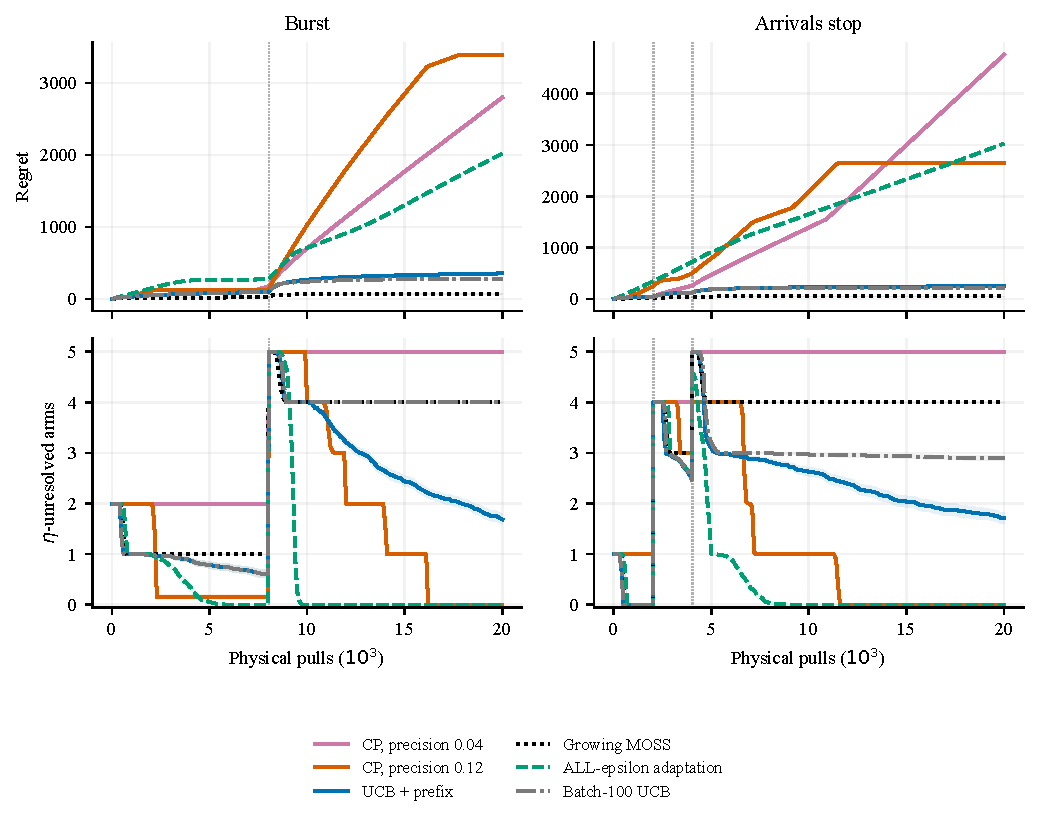
\includegraphics[width=.98\textwidth]{figures/fig_paths_pair2.pdf}
\caption{Additional paths for the burst and stopped-arrival environments.
The six displayed policies, common potential reward streams, 160
replications, and 1.96 Monte Carlo standard error bands are the same as
in the main path figure. Vertical lines mark actual arrivals. The full
run-level data and saved paths retain all nine policies.}
\label{fig:paths-additional}
\end{figure}

\subsection{Admission and reward-retirement accounting}

Let $\mathcal A_t^{\rm adm}\subseteq\mathcal A_t$ be the arms admitted
for reward selection, and let $B_t\subseteq\mathcal A_t^{\rm adm}$ be
its nonempty reward-active subset. Assume $I_t\in B_t$. Adding and
subtracting the admitted and active best means at each physical pull gives
the pathwise identity
\begin{equation}
\begin{aligned}
R_T={}&\sum_{t\le T}\bigl(\max_{i\in B_t}r_i-r_{I_t}\bigr)\\
&+\sum_{t\le T}\bigl(r^*(t)-\max_{i\in\mathcal A_t^{\rm adm}}r_i\bigr)
+\sum_{t\le T}\bigl(\max_{i\in\mathcal A_t^{\rm adm}}r_i
                         -\max_{i\in B_t}r_i\bigr).
\end{aligned}
\label{eq:three_part}
\end{equation}
The components are within-active learning, admission delay, and the
historical-retirement deficit. They are all nonnegative. In Batch100-UCB,
admission occurs at pulls $1,101,201,\ldots$, before action selection.
Reward retirement uses the confidence comparison among currently
admitted active arms after the current observation. Reporting continues
to cover all physically arrived arms, with $[0,1]$ intervals before
admission. Neither waiting for admission nor reward retirement is itself
a certificate of membership or nonmembership in the near-optimal set.

For Checkpoint-UCB, every arrived arm is immediately reward-eligible,
and negative reporting does not remove it from reward selection.
Thus $B_t=\mathcal A_t^{\rm adm}=\mathcal A_t$, so the last two
components vanish identically. The same statement applies to the other
immediate-admission methods that retain every arm for reward selection.

In the Batch100-UCB records, the admission contributions are $0$, $33.92$,
$16.00$, and $22.40$ for the stable, improving, burst, and stopped-arrival
environments, respectively. No retirement deficit occurred. Across all
5,760 records, the largest absolute difference between regret and the
sum in \eqref{eq:three_part} is below $3.1\times10^{-12}$.

\subsection{Verification and computational resources}

The production manifest records Python 3.11.7, NumPy 1.26.4, Numba 0.59.0,
Windows 10, and 13.5 seconds for production generation and recording,
excluding initial compilation and subsequent plotting. The resource snapshot records
20 physical CPU cores, 28 logical cores, and 31.71 GB system memory.
The small physical-round loops use compiled CPU execution. A detected GPU
was not needed. Dependencies and hashes of the reference implementation,
driver, configuration, and numerical records accompany the materials.

The saved production parity check compared the compiled FIFO procedure
with the reference interface for 20,000 consecutive rounds, checking
actions, service indicators, available-arm counts, and reports. That is a
historical implementation check. In this revision, separate short
deterministic checks compare the same interfaces around arrivals, quota
crossings, frozen intervals, and negative reports. The revision also
recomputes the 24 main-table rows, the complete allocation table, and the
640 all-unresolved finer-checkpoint records from the saved data.
These operations leave the simulation records and policy code unchanged.
They are implementation and accounting checks, rather than new method
comparisons or probability certificates.

The local materials support these resource and reproducibility
descriptions. A public repository or permanent release identifier has not
been verified for this version.


\FloatBarrier
\bibliographystyle{plainnat}
\bibliography{references}
\end{document}
